% Koko
\documentclass[ichigo,normal,cn]{elegantnote_mod}
\usepackage{tikz}
\usetikzlibrary{shapes,snakes}
\newfontfamily\courier{Courier New}
\lstset{linewidth=1.1\textwidth,
	numbers=left,
	basicstyle=\small\courier,
	numberstyle=\tiny\courier,
	keywordstyle=\color{blue}\courier,
	commentstyle=\it\color[cmyk]{1,0,1,0}\courier, 
	stringstyle=\it\color[RGB]{128,0,0}\courier,
	frame=single,
	backgroundcolor=\color[RGB]{245,245,244},
	breaklines,
	extendedchars=false, 
	xleftmargin=2em,xrightmargin=2em, aboveskip=1em,
	tabsize=4, 
	showspaces=false
	basicstyle=\small\courier
}
\title{网球循环赛日程表设计}
\author{2017211305 班 \\ 2017211240 于海鑫}

\begin{document}
\maketitle

\section{题目描述}

设有 $n$ 个运动员要进行网球循环赛。
设计一个满足下列条件的比赛日程表:
\begin{itemize}
    \item 每个选手必须与其他 $n-1$ 个选手各赛一次
    \item 每个选手一天只能赛一次
    \item 当 $n$ 是偶数时,循环赛进行 $n-1$ 天
    \item 当 $n$ 是奇数时,循环赛进行 $n$ 天
\end{itemize}

\section{简化版本}

在尝试解决原本的问题之前,我们先考虑一个更加严格,解答起来也更加
简单的问题。我们可以(暂时地)把 $n$ 限制为 $2^k$,其中 $k \in Z$。
此时使用分支求解该问题时问题可以均匀的划分,降低求解的难度。例如,图~\ref{fig:Tour}~
是当运动员数目为 8 时候日程表之一。

\begin{figure}[!htbp]
    \centering
    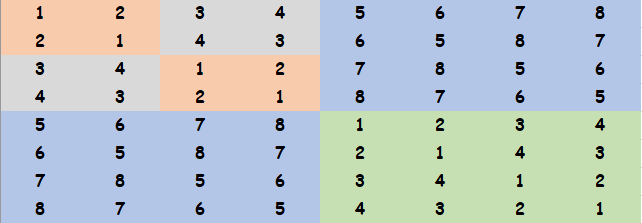
\includegraphics[width=.8\textwidth]{fig-1}
    \caption{循环赛日程表示例}
    \label{fig:Tour}
\end{figure}

不难发现,在这种情况下,将子问题的解直接复制到対角问题就
可以直接得到原问题的解。

\begin{lstlisting}{language=python}
from typing import *


def tourment(p: int, q: int, size: int, array: List[List[int]]) -> None:

    # 当矩阵大于 4 时,对左上角以及右上角分别求解
    if size > 3:
        tourment(p, q, size // 2, array)
        tourment(p, q + size // 2, size // 2, array)

    # 将结果复制到矩阵的下半部分
    for i in range(p + size // 2, p + size):
        for j in range(q, q + size // 2):
            array[i][j] = array[i - size // 2][j + size // 2]
        for j in range(q + size // 2, q + size):
            array[i][j] = array[i - size // 2][j - size // 2]


def print_matrix(matrix: List[List[int]]) -> None:
    print('[')
    for i in matrix:
        print(i)
    print(']')


def solve(k: int) -> List[List[int]]:
    n = 2 ** k
    result = []

    for j in range(n):
        result.append([i + 1 for i in range(n)])
    tourment(0, 0, n, result)
    print_matrix(result)
    return result


if __name__ == '__main__':
    solve(3)

\end{lstlisting}

测试结果如下:

\begin{lstlisting}
PS C:\Users\name1\Desktop> python .\t.py
[
[1, 2, 3, 4, 5, 6, 7, 8]
[2, 1, 4, 3, 6, 5, 8, 7]
[3, 4, 1, 2, 7, 8, 5, 6]
[4, 3, 2, 1, 8, 7, 6, 5]
[5, 6, 7, 8, 1, 2, 3, 4]
[6, 5, 8, 7, 2, 1, 4, 3]
[7, 8, 5, 6, 3, 4, 1, 2]
[8, 7, 6, 5, 4, 3, 2, 1]
]
\end{lstlisting}

与示例完全一致。

\section{求解原问题}
\subsection{初始思路}
在取消 $n$ 的长度限制后,我们首先会想到的解法显然就是补齐参赛选手人数
到 $2^k$,继续使用上面的简化版本代码。在最后删除掉我们补上去的``虚拟选手'',
其伪代码如下:

\begin{lstlisting}{language=python}
from math import log2
def solve_1(n: int) -> List[List[int]]:
    result = solve(log2(n) + 1)
    do_remove_virtual(result)
    return result
\end{lstlisting}

不幸的是,尽管该办法可以保证每个人都只进行 $n - 1$ 次比赛,但是总的比赛
天数还是 $2^k - 1$ 天。我们需要更聪明的方式来处理这一问题。

\subsection{优化}
我们依然使用 ``虚拟选手'' 的方法来解决这个问题,不过与上面那个比较 ``naive'' 的思路
相比,这次我们只在分治遇到规模为 $2k - 1$ 的问题时才添加一个``虚拟选手'',
这样我们在合并过程中就可以很简单地消除掉``虚拟选手''对总体天数的影响。我们选取的
消除``虚拟选手''的方法为:前 $\frac{n}{2}$ 轮比赛中与虚拟选手比赛的与下一个未参赛的选手进行比赛。

代码如下:

\begin{lstlisting}{language=python}
from typing import *


def tourment(size: int, result: List[List[int]]) -> None:
    if size == 1:
        result[1][1] = 1
    elif size % 2 != 0:
        tourment(size + 1, result)
    else:
        tourment(size // 2, result)
        copy(size, result)


def copy(size: int, result: List[List[int]]) -> None:
    if size > 2 and (size // 2) % 2 != 0:
        cp_odd(size, result)
    else:
        cp_even(size, result)


def cp_even(size: int, result: List[List[int]]) -> None:
    mid = size // 2
    for i in range(1, mid + 1):
        for j in range(1, mid + 1):
            result[i][j + mid] = result[i][j] + mid
            result[i + mid][j] = result[i][j + mid]
            result[i + mid][j + mid] = result[i][j]


def cp_odd(size: int, result: List[List[int]]) -> None:
    temp = [0 for _ in range(size + 1)]
    mid = size // 2

    for i in range(1, mid + 1):
        temp[i] = mid + i
        temp[mid + i] = temp[i]

    for i in range(1, mid + 1):
        for j in range(1, mid + 2):
            if result[i][j] > mid:
                result[i][j] = temp[i]
                result[mid + i][j] = (temp[i] + mid) % size
            else:
                result[mid + i][j] = result[i][j] + mid

        for j in range(2, mid + 1):
            result[i][j + mid] = temp[i + j - 1]
            result[temp[i + j - 1]][j + mid] = i


def print_matrix(matrix: List[List[int]]) -> None:
    print('[')
    for i in matrix:
        print(i)
    print(']')


def strip(size: int, matrix: List[List[int]]) -> List[List[int]]:
    result = []
    for i in range(1, size + 1):
        tmp = []
        for j in range(1, size + 1 if size % 2 == 0 else size + 2):
            tmp.append(matrix[i][j] if matrix[i][j] <= size else 0)

        result.append(tmp)

    return result


def solve(n: int) -> List[List[int]]:
    result = []

    for j in range(n + 2):
        result.append([0 for _ in range(n + 2)])
    tourment(n, result)
    result = strip(n, result)
    print_matrix(result)


if __name__ == '__main__':
    solve(6)
\end{lstlisting}

运行结果如下:

\begin{lstlisting}{language=python}
PS C:\Users\name1\Desktop> python .\fft.py
[
[1, 2, 3, 4, 5, 6]
[2, 1, 5, 3, 6, 4]
[3, 6, 1, 2, 4, 5]
[4, 5, 6, 1, 3, 2]
[5, 4, 2, 6, 1, 3]
[6, 3, 4, 5, 2, 1]
]
\end{lstlisting}

与推算结果一致。

\subsubsection{复杂度分析}

显然,有
$$T(n) = T(\frac{n}{2}) + \frac{n^2}{4}$$

因此,由主定理,我们知道
$$T(n) = \Theta(n^2)$$

\subsection{非分治解法}

实际上,这个问题我们还可以使用时间复杂度也是 $\Theta(n^2)$ 的
多边形轮转法解决,但是该解法不在本作业的讨论范围内。

\end{document}